% This file was created by matlab2tikz.
%
\definecolor{mycolor1}{rgb}{0.85000,0.32500,0.09800}%
\definecolor{mycolor2}{rgb}{0.00000,0.44700,0.74100}%
%
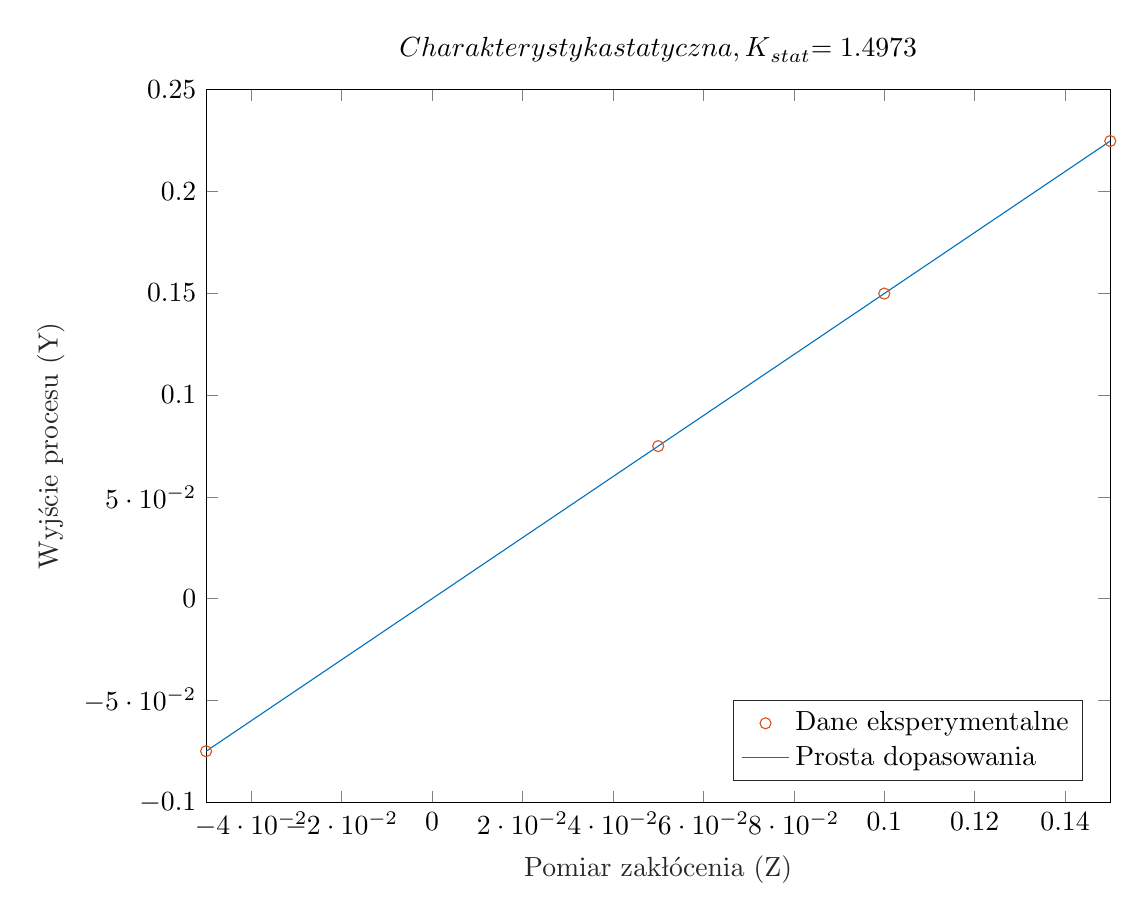
\begin{tikzpicture}

\begin{axis}[%
width=4.521in,
height=3.566in,
at={(0.758in,0.481in)},
scale only axis,
xmin=-0.05,
xmax=0.15,
xlabel style={font=\color{white!15!black}},
xlabel={Pomiar zakłócenia (Z)},
ymin=-0.1,
ymax=0.25,
ylabel style={font=\color{white!15!black}},
ylabel={Wyjście procesu (Y)},
axis background/.style={fill=white},
title style={font=\bfseries},
title={$\text{Charakterystyka statyczna, K}_{\text{stat}}\text{ = 1.4973}$},
legend style={at={(0.97,0.03)}, anchor=south east, legend cell align=left, align=left, draw=white!15!black}
]
\addplot [color=mycolor1, only marks, mark=o, mark options={solid, mycolor1}]
  table[row sep=crcr]{%
0.05	0.0748666667701207\\
0.1	0.149733333540241\\
0.15	0.224600000310365\\
-0.05	-0.0748666667701207\\
};
\addlegendentry{Dane eksperymentalne}

\addplot [color=mycolor2]
  table[row sep=crcr]{%
-0.05	-0.0748666667701214\\
-0.04	-0.0598933334160971\\
-0.03	-0.0449200000620728\\
-0.02	-0.0299466667080486\\
-0.01	-0.0149733333540243\\
0	0\\
0.01	0.0149733333540243\\
0.02	0.0299466667080486\\
0.03	0.0449200000620728\\
0.04	0.0598933334160971\\
0.05	0.0748666667701214\\
0.06	0.0898400001241457\\
0.07	0.10481333347817\\
0.08	0.119786666832194\\
0.09	0.134760000186218\\
0.1	0.149733333540243\\
0.11	0.164706666894267\\
0.12	0.179680000248291\\
0.13	0.194653333602316\\
0.14	0.20962666695634\\
0.15	0.224600000310364\\
};
\addlegendentry{Prosta dopasowania}

\end{axis}
\end{tikzpicture}%